% --------------------------------------------------------------
% This is all preamble stuff that you don't have to worry about.
% Head down to where it says "Start here"
% --------------------------------------------------------------
 
\documentclass[12pt]{article}
 
\usepackage[margin=1in]{geometry} 
\usepackage{amsmath,amsthm,amssymb, graphicx}
 \usepackage{algorithm}
\usepackage{algorithmic}

\newcommand{\N}{\mathbb{N}}
\newcommand{\Z}{\mathbb{Z}}
 
\newenvironment{theorem}[2][Theorem]{\begin{trivlist}
\item[\hskip \labelsep {\bfseries #1}\hskip \labelsep {\bfseries #2.}]}{\end{trivlist}}
\newenvironment{lemma}[2][Lemma]{\begin{trivlist}
\item[\hskip \labelsep {\bfseries #1}\hskip \labelsep {\bfseries #2.}]}{\end{trivlist}}
\newenvironment{exercise}[2][Exercise]{\begin{trivlist}
\item[\hskip \labelsep {\bfseries #1}\hskip \labelsep {\bfseries #2.}]}{\end{trivlist}}
\newenvironment{problem}[2][Problem]{\begin{trivlist}
\item[\hskip \labelsep {\bfseries #1}\hskip \labelsep {\bfseries #2.}]}{\end{trivlist}}
\newenvironment{question}[2][Question]{\begin{trivlist}
\item[\hskip \labelsep {\bfseries #1}\hskip \labelsep {\bfseries #2.}]}{\end{trivlist}}
\newenvironment{corollary}[2][Corollary]{\begin{trivlist}
\item[\hskip \labelsep {\bfseries #1}\hskip \labelsep {\bfseries #2.}]}{\end{trivlist}}

\newenvironment{solution}{\begin{proof}[Solution]}{\end{proof}}
 
\begin{document}
 
% --------------------------------------------------------------
%                         Start here
% --------------------------------------------------------------
 
 
% Your write-up should contain:
% the names of the people in your group (and each member's contribution),
% the optimizations used or attempted,
% the results of those optimizations,
% the reason for any odd behavior (e.g., dips) in performance, and
% how the performance changed when running your optimized code on a different machine. 
\title{CS 267 Homework 1 Part 1}
\author{Xingyou Song \footnote{xsong@berkeley.edu - Xingyou wrote the report, presented techniques and strategies for optimization, and coded some parts}, Yao Yuan \footnote{yao\_yuan@berkeley.edu - Yao coded a significant part of the code in C and tested using various compiler settings} \footnote{Our Third Partner, Zhiwei Yao, dropped the course.}} %replace with your name
\date{Due Feburary 9, 2018} 
\maketitle

\section{General Optimizations}
For almost all of our trials and codes, we tried common techniques. Ultimately we specifically tailored each of these methods for different implementations, however. 

\subsection{Switching for loop variables}
Note that in the original code, the main code within the 3 nested loops (for do\_block, and to a magnified extent, square\_dgemm) was: $C[i,j] += A[i,k] * B[k,j]$. The original order for the nested do\_block function was, from outer to inner order: $i,j,k$. For the $B$ matrix, this ordering moved the entries downward on the columns of $B$, but moved the entries row-wise on $A$, which was cache-inefficient. By instead using $j,k,i$ ordering, this also allowed the $i$ variable to move downwards on the columns of $A$. This inspired essentially ways to reorganize the for loops to allow for better cache access. 

\subsection{Buffer Copying} 
Because the do\_block function uses blocks of matrices $A,B,C$, this leads to only columns of a block being consecutive in memory, which leads to redundant cache loads (i.e. a cache line may be much longer than the column size of a block). Thus, every time we used the do\_block function, we would load in the input A-block and B-blocks into temporary contiguous memory.  
\subsubsection{Transposition of A-blocks}
While copying, we also considered transposition of the elements for a given A-block, allowing the A-block to be row-major in temporary memory. This would allow the writes to be consecutive: $C[i,j] += A[i, 1]*B[1, j], C[i,j] += A[i,2]* B[2, j],...$ 
\subsubsection{Padding}
To allow for cache-alignment, we also padded 0's into the buffers. Cache alignment allows for consecutive address access, to prevent any cache-misses. 

\subsection{Vectorization} 
To allow for the Intel compiler to detect vectorization,  we unrolled parts of computation within the inner-most loop. In theory, this should allow the compiler to use the AVX 4-vector commands, as well as its FMA (Fused Multiply-Add) operation for speedup. In code, this would mean unrolling loops in order for the inner-most portion to have multiply and add operations on 4, consecutive doubles in memory.

\subsection{Parameter Tuning}
The above methods imply that the size-parameters (for block sizes) must be carefully adjusted. Essentially, there should be a balance among the following aspects: 
\begin{enumerate}
\item Larger copies are expensive because of more memory operations, as reading from memory is expensive, with writing even more expensive.
\item The parameters should be fine tuned in order to match with the $L1, L2$ cache sizes (both total memory sizes and cache-line lengths). L1 cache is considered when making a second blocking function (e.g. do\_block\_L1 inside do\_block). 
\item Having too low block sizes generates more overhead overall, and especially for boundary mismatches (for cache lines as well as inner blocking functions).  
\end{enumerate}

\subsection{Code Tweaks}
We also made small code improvements that sometimes improved performance by small increments. These include: 
\begin{itemize}
\item Removing redundant calculations (e.g. removing a line out of a for-loop if it remains constant over the entire loop)
\item Preprocessing calculations - Since multiplications are relatively expensive, it makes sense to only precalculate an index $(i +j* stride)$ once, store this value, and use it as often as possible. 
\end{itemize}


\section{(Submitted) dgemm-blocked.c }
\subsection{Performance}
Overall, our submission gave an average of $44 \%$ over the normal test cases. Note that the asymptotic performance is above $50 \%$ for large matrices, while there is less performance for smaller matrices. The major explanation for this is due to the use of the transpose function on $A$ early on, rather than later - This gives a large boost for larger matrices than it does for smaller matrices.    
\begin{figure}[h]
  \caption{Performance for our submission vs. BLAS}
  \centering
    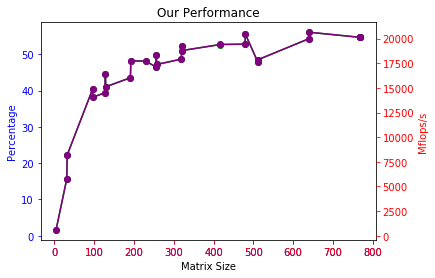
\includegraphics[width=0.6\textwidth]{our_performance_graph.png}
     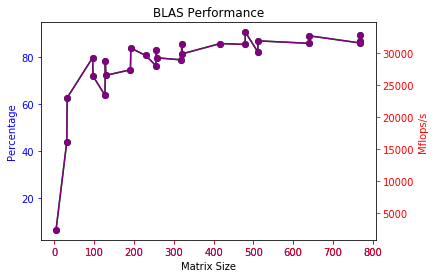
\includegraphics[width=0.6\textwidth]{blas_performance_graph.png}
\end{figure}
\subsection{Methods}
Our submission consists of the following functions:
\begin{itemize}
\item weird\_transformation - This transforms the input matrix by stretching its columns by STRIDE times, while reducing its rows by STRIDE times (and padding the last row accordingly if there is uneven divisibility).
\item compute - This performs AVX vectorization to update each 8x4 block of the C-matrix, given input as "smaller blocks", using the FMA intrinsic. 
\item do\_block\_large - This cuts an input block into smaller blocks, with each smaller block passed into compute. 
\item square\_dgemm - This cuts the entire matrix inputs into blocks to be passed into do\_block\_large. 
\item vectorized\_FMA - This takes in 8x4 matrix from C and performs the correct updates. 
\end{itemize}
Note that the ordering of the 3 nested for loops in each of the functions (square\_dgemm, do\_block\_large, compute) are subtly not the same. For notation purposes (i.e. i,j,k representing columns and rows), suppose that computation is always performed using the update rule (where $C[i,j]$ may represent a larger block, smaller block, or individual element): $C[i,j] += A[i, k]*B[k, j]$. Furthermore, we may define, roughly speaking, 'large blocks' data intended to fit in L2 cache, while "small blocks" data intended to fit in L1 cache. The 8x4 AVX vectorization is therefore intended for the CPU registers. 

Then we have the following orderings: 
\begin{itemize}
\item square\_dgemm is in i-j-k ordering. The reason for this is to fill in a large block of $C$ in one pass as the data is in L2, to prevent too many DRAM passes if we kept making passes over larger blocks in intervals.  
\item do\_block\_large is in k-j-i ordering. Because A has been made row major early on, this allows cache lines to also follow the order of the blocking movement of A. 
\item compute is in i-j-k ordering. This is also explained by the fact that i must be before j for AVX memory loads from the C matrix, with k moving consecutively. 
\end{itemize}

Thus the pseudocode for the algorithm is presented below (ignoring boundary cases, small tweaks, etc.) 

\begin{algorithm}
\caption{SQUARE-DGEMM(lda, A,B,C)}
\begin{algorithmic} 
\STATE $A_{weird} \leftarrow weird\_transformation(A)$

\STATE $LARGE\_M = 128$
\STATE $LARGE\_N = 256$
\STATE $LARGE\_K = 512$

\FOR{$i=0, i<lda, i+= LARGE\_M$}
\FOR{$j=0, j<lda, j+= LARGE\_N$}
\FOR{$k=0, k<lda, k+= LARGE\_K$}



\STATE do\_block\_large(block(i,j,k) )

\ENDFOR
\ENDFOR
\ENDFOR
\end{algorithmic}
\end{algorithm}

\begin{algorithm}
\caption{do\_block\_large(M, N, K)}
\begin{algorithmic} 
\STATE $A_{weird} \leftarrow weird\_transformation(A)$

\STATE $SMALL\_M = 128$
\STATE $SMALL\_N = 128$
\STATE $SMALL\_K = 128$

\FOR{$k=0, k<K, k+= SMALL\_K$}
\FOR{$j=0, j<N, j+= SMALL\_N$}
\FOR{$i=0, i<M, i+= SMALL\_M$}

\STATE compute(small\_block($i,j,k$))

\ENDFOR
\ENDFOR
\ENDFOR
\end{algorithmic}
\end{algorithm}

\begin{algorithm}
\caption{compute(M, N, K)}
\begin{algorithmic} 


\FOR{$i=0, i<M, i+= 8$ }
\FOR{$j=0, j<N, j+= 4$}

\STATE Vectorized\_FMA($8 \times 4$ $C_{i,j}$)

\ENDFOR
\ENDFOR
\end{algorithmic}
\end{algorithm}

\newpage 
\subsection{Performance On Local Computer}
We performed the same code on a personal laptop, Lenovo Y510p with Intel i7 4700MQ 2.4 GHz, which allows AVX/AVX2 instructions. It also had the same cache specifications as Cori. The CPU allows for maximum frequency 3.4 GHz, but this was disabled. Thus this implies that the theoretical optimum is 2.4 GHz * 8 vector width * 2 flops for FMA = 38.4 GF/s, similar to the benchmark on Cori as well. This gave an average of 53 \% over all test trials, with more percentages given larger matrix sizes. 
\begin{figure}[h]
  \caption{Performance for our submission on local computer (Lenovo Y510p)}
  \centering
    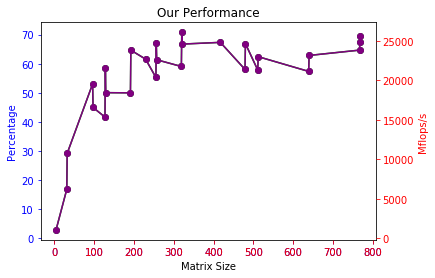
\includegraphics[width=0.6\textwidth]{our_performance_graph_lenovo.png}
\end{figure}
The performance seemed to be slightly better than Cori - this is possibly due to using the GCC compiler rather than the ICC compiler, as this is the only significant difference between the two machines. 


\section{Other Methods Considered}
In this section, we briefly describe some of the other methods which failed, as well as how our code's performance progressed as we added more features. Note that some of the other trials performed approximately 20\% on smaller test cases, such as sizes 1-32, while our code performs poorly on smaller sizes. This is expected, because our submission performs 2 layers of blocking, which creates a large overhead for small matrices.

\subsection{GEPP} 
One of the methods implemented was a reimplementation of the paper \footnote{Goto, K., and van de Geijn, R. A. 2008. Anatomy of High-Performance Matrix Multiplication, ACM Transactions on Mathematical Software 34, 3, Article 12}, which used recursive functions GEPP and GEBP, which partitioned blocks into columns, which were also sub-partitioned. This implemented the buffer-copying transpose aspect, but was only optimized for the L2-cache. Transposition and manual SSE instructions were also implemented in a 4x4 fashion. Ultimately however, this achieved only 16\% - 20\% average performance on the Cori supercomputer. The cause of this failure might have been due to lack of usage of the FMA instructions, as well as disregard for the L1 cache. 

\subsection{SSE-4x4, 2x2}
SSE instructions were also used for vectorizing two doubles ignoring L1 cache optimization and transpose., early on for the code. A blocked kernel of size 4x4 and 2x2's were used. Unfortunately, this also only achieved approximately 14 \%. It seemed that use of the L1 cache is highly critical to optimization. Furthermore, any further optimizations for loops \textbf{other} than $i-j-k$ ordering for calling do\_block had a very large overhead for DRAM access, which enforced that every block of matrix C needed to be filled immediately. 
 
% --------------------------------------------------------------
%     You don't have to mess with anything below this line.
% --------------------------------------------------------------
 
\end{document}
